\graphicspath{{./}{./figures/}{./figures/background/}}

\section{Audio Synthesizers}
In the context of audio, a synthesizer refers to a device that generates sound or music. Martin Russ provides a thorough overview of audio synthesis in his textbook, Sound Synthesis and Sampling \cite{russ2012sound}. Russ introduces the synthesizer as any device that gerates sound,  even the human voice can be thought of as a synthesizer, however, sound synthesizers have become more broadly accepted as an electronic device that produces synthetic sounds. A synthesizer may do this through the playback and recombination of pre-existing audio material or through the generation of raw audio waveforms. There are numerous types of synthesis techniques that are capable of producing a huge variety of different sounds. Broadly speaking, these sounds can be categorized into two different classes: `imitative` or `synthetic`. Imitative sounds attempt to emulate a sound that exists in the natural world such as a physical musical instrument or a sound effect such as an explosion. Electric pianos are examples of imitative synthesizers. Synthetic sounds are those that have no relation to a sound in the physical world. The distinction between imitative and synthetic sounds is blurry and most sounds fall somewhere in the middle. For example, synth-brass sounds, which were a staple of synths such as Roland's popular Jupiter-8, are sounds that are based on an imitation of a brass sound but extend into the synthetic realm. 

% This is maybe a bit more like introduction material?
Synthesizers have become ubiquitous in audio production and entire genres of music have been developed around their use. Bebe and Louis Barron produced the first electronic film score for the movie "Forbidden Planet" in 1955 using synthetic sounds. Since then the use of synthesizers for movies and video games has also become common-place.


\subsection{Evolution of Synthesizers}
A brief history of synthesizers is provided here for historical context to the development and use of synthesizers. The full history of the topic is beyond the scope of this thesis and the interested reader is referred to some great textbooks that cover audio synthesizers and their history \cite{roads1980interview, mcguire2015musical, jenkins2019analog, russ2012sound}, which were used in the writing of this chapter.
\subsubsection{Analog}
Until the late 1950s all synthesizers were analog. All analog synthesizers are defined by their use of continuous-time signals, as opposed to digital systems which operate in discrete chunks of information, or discrete-time signals. Early analog synthesizers can be broken down into two broad categories: (1) sounds that are generated directly by electric circuits by oscillating vaccuum tubes, or (2) rotating or vibrating physical systems that are controlled by electronic sources \cite{roads1996computer}. The first, as well as the largest sound synthesizer ever built was developed in the early 1900s by Thaddeus Cahill. On September 26, 1906, an audience of 900 individuals came to view the massive electronic instrument called the Telharmonium that was capable of producing pure sinusoidal waves in at frequencies in integer ratios. Other early synthesizers include the Theremin, built by Leon Theremin in 1920, which produced a pure tone with a varying pitch and amplitude that was controlled by a performer moving their arms in relation to two antennas. The sound produced by the theremin has an eery feel to it, well-suited for sci-fi film scores. Versions of the theremin have been used in popular music by musicians including The Beach Boys, Led Zeppelin, and The Rolling Stones (citations? check out wikpedia).  The Ondes Martenot, developed in 1928 by Maurice Martenot and Ondes, had a similar sound to the theremin and also was one of the first synthesizers to include a piano-like keyboard interface.

In the 1960s two companies emerged on opposite sides of America and released synthesizers that have shaped the landscape of audio synthesis. Around 1964 Don Buchla, who lived in the San Francisco area, released the the Buchla 100 Series Modular Electronic Music System and Robert Moog, who lived in the New York area, released the R.A. Moog Modular System \cite{mcguire2015musical}. Both synthesizers were modular systems that had individual processing units called \textit{modules} that could be interconnected using patch cables, connecting together synthesizer modules is known as creating a "synth patch", or simply a "patch". Both systems also include Voltage-Controlled Oscillators (VCOs) which create electronic waveforms at stable musical pitches, and the pitch can be controlled via an input signal. The Moog Modular System also featured a Voltage Controlled Filter (VCF) that was an early version of Moog's famous ladder filter design that would resonate at a controllable center frequency, creating some of the most iconic synthesizer sounds that are still used today.

There were some important philosophical differences between Moog and Buchla Synthesizers that have lead to two different schools of thought: East Coast and West Coast synthesis. The development of the Buchla synthesizer by Don Buchla was guided by Morton Subotnick and other experimental composers working out the San Francisco Tape Music Center. Subotnick explicitly requested that the synthesizer was not controlled by a traditional keyboard interface as he was worried that it would trap him into created tonal music. Instead, Buchla synthesizers are controlled using a set of touch plates and sequencers. At the same time on East coast Robert Moog was developing the Moog Modular and building a traditional keyboard interface to control the pitch of his VCOs. This feature, which allowed the Moog Modular Systems to be integrated more easily with Western music, was one of the reasons that Moog synthesizers became much more popular and commercially successful compared to Buchla. 

Another reason that Moog synthesizers were launched into the public eye is because of their use in recorded music. In 1968 Wendy Carlos used a Moog Modular synthesizer to orchestrate, perform, and record a selection of Johann Sebastian Bach pieces. The collection of music, called \textit{Switched On Bach}, went on to become the best selling classical recording of all time. Other musicians had created recreations of classical music pieces on synthesizers, but none had reached the same level as \textit{Switch On Bach}. Jenkins \cite{jenkins2019analog} credits the nature of the counterpoint in Bach's pieces as being particularly well suited to synthesizers, as well as Carlos' ability to design sounds that brought that performance alive, to the success of the release. Building on this success Carlos went on to score synthesized soundtracks for movies including Stanley Kubrick's \textit{A Clockwork Orange}. Another exceptional example of classical music recreated using Moog synthesizers worth mentioning is Japanese composer Isao Tomita's \textit{Snowflakes Are Dancing}, which was released in 1974. The use of synthesizers in music and film extends into almost all genres of music and was the cornerstone in the development of new genres including techno and other electronic music genres. [Also note something about the historical context and other synthesizer manufacturers] -> Mark Jenkins provides an excellent overview of the use of synthesizers in various genres of music over the years in his book \textit{Analog Synthesizers: Understanding, Performing, Buying} \cite{jenkins2019analog}.

\subsubsection{Digital}
The first experiments with digit synthesis were conducted by Max Mathews on an IBM 704 computer in 1957 \cite{roads1980interview}. These experiments consisted of programming and synthesizing melodies using triangle waves, Mathew's program was able to accept the note pitch, amplitude, and duration. The Music III program was developed by Mathew's in 1960 and introduced an important concept called the \textit{unit generator}, which defined basic components of a synthesizer in programmatic units that a user was able to link together to create a full synthesizer architecture. Mathew's describes these concepts as being developed in parallel, but separately, to similar synthesis concepts (e.g. modular synthesizers) being developed in the analog world. He described this as "an advantage because a musician who knew who to patch together Moog synthesizer units would have a pretty good idea how to put together unit generators in the computer."

In 1973 John Chowning, a researcher at Stanford, released a landmark audio synthesis paper entitled on Frequency Modulation (FM) synthesis \cite{chowning1973synthesis}. The patent for FM synthesis was licensed to Yamaha who developed the Yamaha DX7 synthesizer using the technology, which was released in 1983 and became one of the best selling synthesizers of all time. One of the major benefits of FM synthesis is that it is able to produce complex audio waveforms at low computational cost. Additionally, the Yamaha DX7 was a fully polyphonic synthesizer, meaning that it was capable of producing multiple tones simultaneously (i.e. was able to play chords), whereas most analog synthesizers that were within the same time period were monophonic (only capable of playing one note at a time). The Yamaha DX7 was also incredibly difficult to program, although it came preloaded with a large selection of quality parameter settings, or presets, that allowed users to play the synth without have to learn how to program it.

As digital technology improved and computers became more powerful, new synthesis techniques such a sampling synthesis \cite{mcguire2015musical} and physical modelling \cite{jaffe1983extensions} emerged. Digital emulations of analog synthesizers, or virtual analog (VA) synthesis, also started to become popular in the 1990s. VA synthesizers attempt to express traditional analog synthesis methods in code as digital signal processing (DSP) algorithms. The development of more powerful computers also enabled recording workflows to be transferred into software and professional recording studios started to transition to digital with the release of Digidesign ProTools in the early 1990s. As software synthesis became more prevalent, many types of different software synthesizers emerged including VA software synthesis and a trend emerged of directly emulating analog equipment digitally, including the user interface. Skeumorphism describes computer user interfaces that attempt directly mimic their real-world counterpoint, and has become extremely common in audio software, including synthesizers; user interface researchers have begun to question whether or not these skeumorphic interfaces enhance usability of not \cite{lindh2018beyond}.

\subsubsection{Audio Plugins}
In 1996 Steinberg\footnote{\url{https://www.steinberg.net}} released the Virtual Studio Technology (VST) interface, which allowed third-party software including audio effects to be integrated into host applications including DAWs. Because VSTs integrate with host applications, they are also called audio plug-ins. The second version of VST was released in 1999 which added support for the Musical Instrument Digital Interface (MIDI) \cite{rothstein1992midi}, a communication protocol enabling musical hardware and software to exchange information and control signals. The addition of MIDI to the VST interface opened the doors for VSTi, VST instruments, including software synthesizers. Other audio plug-in architectures have been developed in addition to VSTs, and popular ones include Apple's Audio Units (AU) and Avid's Avid Audio eXtension (AAX). Audio plug-ins have allowed software developers a method to create unique audio effects and synthesizers, and an industry dedicated to their development has blossomed over the last few decades. At the time of writing there are over 500 different synthesizer plug-ins available for purchase or for free on the KVR\footnote{\url{https://www.kvraudio.com/plugins/softsynth-virtual-instruments}} database of audio products.

\subsection{Components of a Synthesizer}
Synthesizers can be viewed as comprising two major components: the synthesis engine, which is where sounds is generated, and a control interface which allows a user to control the synthesis engine \cite{russ2012sound}. Audio synthesis can be a complex process, so there is generally a high-level of abstraction between the synthesis engine and the control interface. The role of the control interface is to present a conceptual model of the synthesizer to a user, which allows the user to express their ideas and modify the synthesis engine. The parameters on the control interface are mapped to components within the synthesis engine, often in non-linear and complex ways. Figure \ref{fig:synth_abstraction} shows a diagram of the general components of a synthesizer and the control interface abstraction layer. The following sections provide more detail on each of the two major components of a synthesizer.

\begin{figure}[ht]
    \centering
    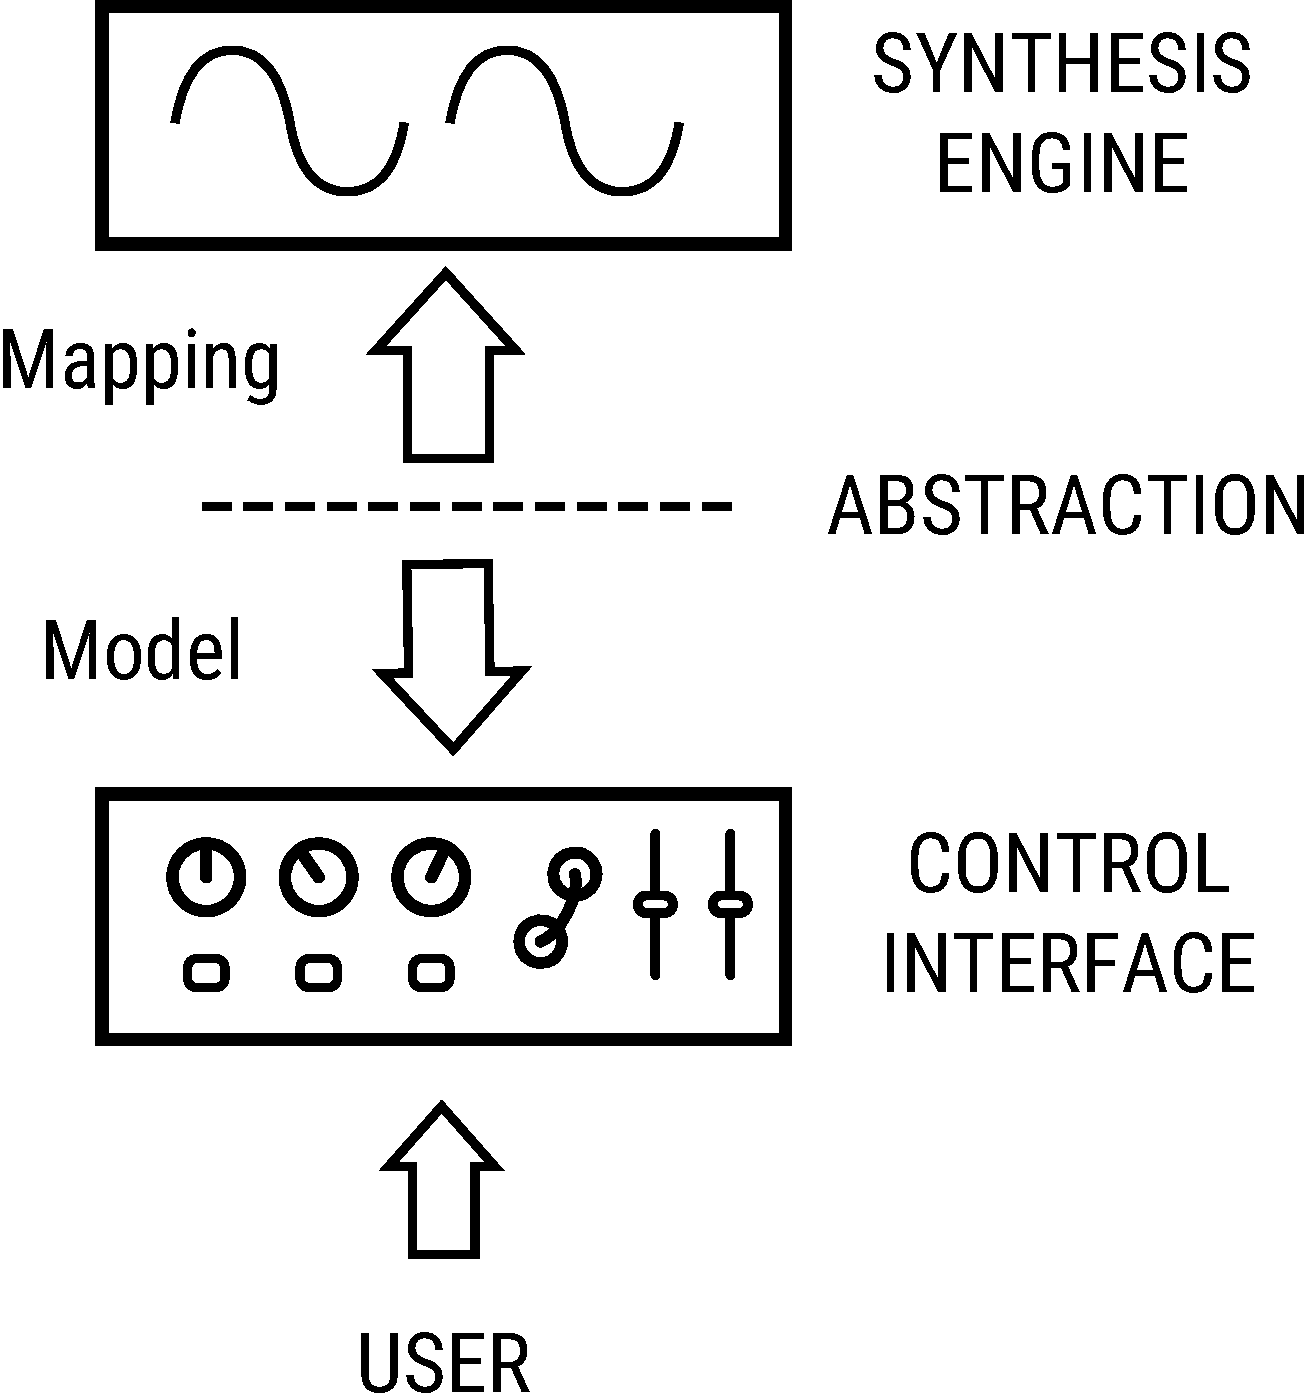
\includegraphics[width=0.4\textwidth]{figures/background/Synth Abstraction Model.pdf}
    \caption{Abstraction between the synthesis engine and control interface. A control interface on a synthesis is responsible for presenting a conceptual model of the underlying synthesis engine to a user. The parameters on the control interface are mapped back to the synthesis engine to modify audio generation.}
    \label{fig:synth_abstraction}
\end{figure}

\subsection{Synthesis Engine}
The synthesis engine is at the heart of sound generation in any synthesizer, whether it is an analog modular synth or a software audio plugin. There have been many different approaches to sound generation, and it is an active field with researchers and audio developers continuing to look for novel ways to create sounds. Sam McGuire and Nathan Van der Rest provide a good overview of some of the more popular synthesis methods in their book \textit{The Musical Art of Synthesis} \cite{mcguire2015musical}. These methods include: subtractive, sample-based, modulation (i.e. FM), additive, wavetable, granular, vector, and physically modelling. 

While the exact technique that each of these methods use may be different, there are some common components to synthesizers that exist in some form across different techniques. It is useful to take a modular perspective when thinking about different synthesizer components, similar to the \textit{unit generator} concept introduce by Max Mathews \cite{roads1980interview}, in which different components of a synthesizer are broken down into functional units (modules) that can be interconnected in various ways. We can generalize modules as all producing some output signal as well as having an optional input signal. Modules may also have some parameters that can be mapped to a control interface to enable user control. We can broadly categorize the signals that are output by modules as either audio signals or control signals. Audio signals are generated by the synthesizer and ultimately are output as a sound. Control signals are used to modulate the parameters of other modules within a synthesizer. In some synthesizers audio signals can also be treated as control signals and be used to modulate parameters of other parameters.

We can categorize modules into two different types based on the type of signal they output: 1) \textbf{audio modules}, generate or process audio signals, and 2), \textbf{control modules}, generate or process control signals. Jenkins provides an overview of some of the different synthesizer modules from the perspective of an analog synthesizer \cite{jenkins2019analog}. In analog synthesis audio signals are commonly generated by voltage-controlled oscillators (VCOs). In a VCO the frequency of the oscillator is controlled by the voltage of an input control signal. While voltages only exist in analog circuits, the concept has been extended into digital synthesizers as well, with the digital equivalent of a VCO sometimes being referred to as a digitally controlled oscillator (DCO). Other common audio modules are voltage-controlled filters (VCFs), voltage-controlled amplifiers (VCAs), and Noise Sources; filters accept audio signals as input and attenuate or boost specific frequencies, VCAs are essentially an automated volume knobs, and noise sources generate different types of noise such as white noise.

Exploring all of these methods in detail is beyond the scope of this thesis, however two methods are particularly relevant to the methods explored: subtractive synthesis and frequency modulation (FM) synthesis. 


\subsubsection{Subtractive Synthesis}
Subtractive synthesis was one of the earliest methods explored and is the sound of the famous Moog synthesizers. It has been used on thousands of records, and is still a popular method. The basic idea behind subtractive synthesis is that the starting point is a harmonically rich waveform, generated by an oscillator, which is then sent through a chain of filters and other audio effects that shape the timbre of the waveform over time. [Insert a simple block diagram of a subtractive synth]. There are several types of waveforms that are generally available on a oscillator in a subtractive synthesizer, these are shown in figure X [insert a diagram of some of the common waveforms and their harmonics]. Each waveform has a unique set of harmonics. Harmonics refer to frequencies that are present in the sound that occur at integer frequency ratios to the fundamental frequency of the sound, which is associated to the perceived pitch of that sound. Sine waves are the simplest waveforms and only contain energy at the fundamental frequency. Noise generators produce energy at all frequencies and contain no fundamental frequency and are therefore inharmonic.

Once a waveform has been generated it may be combined with other waveforms through a process called mixing. The average subtractive synthesizer has three oscillators \cite{russ2012sound} that are typically tuned to harmonically related frequencies. The next common stage in a subtractive synth signal path is an audio filter. As previously mentioned, one of the most famous synthesizer filters of all time is the Moog ladder filter \cite{moog1965voltage}, which is a resonant low pass/high-pass filter. Low pass filters allow low frequency sounds to pass through while attenuating frequencies above a certain threshold frequency, vice-versa for high-pass filters. The threshold frequency is usually controllable and can be modulated using other signals to create dynamic 'sweeping' sounds. After passing through the filter the signal passes through an amplitude gate, which acts as a volume knob that is controlled by an internal control signal envelope. The envelope 



\subsubsection{Frequency Modulation Synthesis}
FM synthesis was an another early method of synthesis that was developed during the origins of digital synthesis methods. FM synthesis engines are capable of produce a huge array of complex waveforms using a relatively simple stucture, which makes them powerful, however more conceptually challenging to understand compared to subtractive methods. The basic unit of an FM synthesizer is referred to as an operator, which generally contains a single simple sine wave oscillator and an amplitude gate controlled by an envelope generator. The simplest FM synthesizer consists of two operators that are connected together in way so that one of the operators controls the frequency of the second operator. The operator that does the modulating is referred to the \textit{modulator} and the operator that is modulated is referred to the \textit{carrier}. [Insert figure showing this arrangement.]

\subsubsection{Neural Synthesis}
One area of new development in audio synthesis is in methods that are leveraging advancements from the field of deep learning [deep learning cite], an area of audio synthesis that is explored in this thesis.  


- Pretty much just give a listing of techniques here. Potentially give a bit more of an overview of substractive vs. FM.
- Sound Synthesis and Sampling provides a thorough overview of both analog and digital synthesizers and the various methods. \cite{russ2012sound}

\subsection{Control Interface}
The control interface presents a conceptual model of the synthesizer to the user and maps this model to the underlying engine. A control interface has a set of parameters that can be altered to modify the nature of the sound being generated. A skilled sound designer is able to interact with the control interface and craft sounds to fit the needs of their creative project. This process is referred to as programming a synthesizer. A well-designed synthesizer control interfaces allow users to build up a conceptual model that allows them to easily interact with the synthesizer in a way that allows them to be expressive. 

% Not so sure about this section.
% The nature of the control interface is guided by the synthesis method being used by the engine. Synthesis methods like subtractive synthesis which involve a clear linear signal flow that starts with a complex waveform that is progressively shaped can lead to a more simple conceptual model. Moog synthesizers are examples of subtractive synthesizers that have clear control interface that maps to the synthesis engine. More complex synthesis methods such as Frequency Modulation (FM) synthesis are more challenging to create clear control maps for. Interestingly, the most commercially successful synthesizer, the Yamaha DX7, had a notoriously difficult control interface, although shipped with an extensive high-quality set of factory presets (pre-defined control interface parameter settings).

\subsection{Synthesizer Programming}
Both Carlos and Tomita excelled at patching synthesizer modules together and tuning the parameters of individual modules to create new sounds to orchestrate their performances. This process ... it's art! Blah blah blah. But also these folks are artists and virtuosos.

- Challenges with synthesizer programming UI design: \cite{seago2013new}. -- "Some, like subtractive synthesis, offer controllers which are broadly intuitive, in that changes to the parameter values produce a proportional and predictable change in the generated sound. Other methods, however, are less easily understood. FM synthesis, for example, is a synthesis method that may be viewed as essentially an exploration of a mathematical expression, but whose parameters have little to do with real-world sound production mechanisms, or with perceived attributes of sound." -- There are some other really good bits about navigating the timbre space and non-linearities.
- \cite{seago2004critical} Thus, under most current systems, the user is obliged to express directives for sound specification in system terminology, rather than in language derived from the user domain. Three types of synthesizer interfaces: parameter selection in a fixed architecture, architecture specification and configuration, and direct specification of physical characteristics of sound.
- Context on synthesizer programming \cite{jenkins2019analog}
- Russ describes the programming component intrinsically creative.
- When we talk about programming synthesizers we are referring to the task of selecting parameter settings for a synthesizer in order to achieve a desired sound
- Talk about the nature of this task. I think in that krekovic study there was something about this process? That this can be done in an exploratory way that ppl enjoy that process.
- Even so, it can still be quite a challenging task.

Programming audio synthesizers is challenging and requires a technical understanding of sound design to fully realize their expressive power. Traditional synthesizers can have over 100 parameters that affect audio generation in complex, non-linear ways. One of the most commercially successful audio synthesizers, the Yamaha DX7, was notoriously challenging to program. Allegedly nine out of ten DX7s coming into workshops for servicing still had their factory presets intact \cite{seago2004critical}.

Give an image of the complex synth UI.

% Bounce this out to another section I think. This could sit in creativity support potentially?
% \subsubsection{Neural Synthesis}
% In contrast to traditional synthesis, neural synthesizers generate audio using large-scale machine learning architectures with millions of parameters \cite{engel2017neural}. Differentiable digital signal processing \cite{engel2020ddsp} bridged the gap between traditional DSP synthesizers with the expressiveness of neural networks, exploring a harmonic model-based approach, using a more compact architecture with 100K parameters.
% One benefit of synthesized audio is that the underlying factors of variation ({\em i.e.}~the parameters) are known.

% % GANs for synthesis
% In this work, we use Generative Adversarial Networks (GANs) \cite{goodfellow2014generative} to generate new instrumental audio from a dataset of existing material. GANs have the potential to be used to generate new sounds on the fly. This would dramatically alleviate both the problem of having to pore through giant sound libraries, and the problem with having to only use one sample repeatedly. In addition, the explosion of new sounds which could potentially be produced by GANs would vastly reduce recording costs by designers of sound libraries.

% This research avenue is to a certain degree untapped: GANs have been successfully applied to the generation and manipulation of images, however, relatively little work has been focused on the audio domain. Research related to the specific work proposed here was presented by \cite{donahue2018adversarial}  and \cite{engel2018gansynth}.

